% ============================================================
% fig_atencion_intuicion.tex — Intuición del mecanismo de atención
% Uso: % ============================================================
% fig_atencion_intuicion.tex — Intuición del mecanismo de atención
% Uso: % ============================================================
% fig_atencion_intuicion.tex — Intuición del mecanismo de atención
% Uso: % ============================================================
% fig_atencion_intuicion.tex — Intuición del mecanismo de atención
% Uso: \input{figures/fig_atencion_intuicion}
% ============================================================
\begin{figure}[H]
\centering
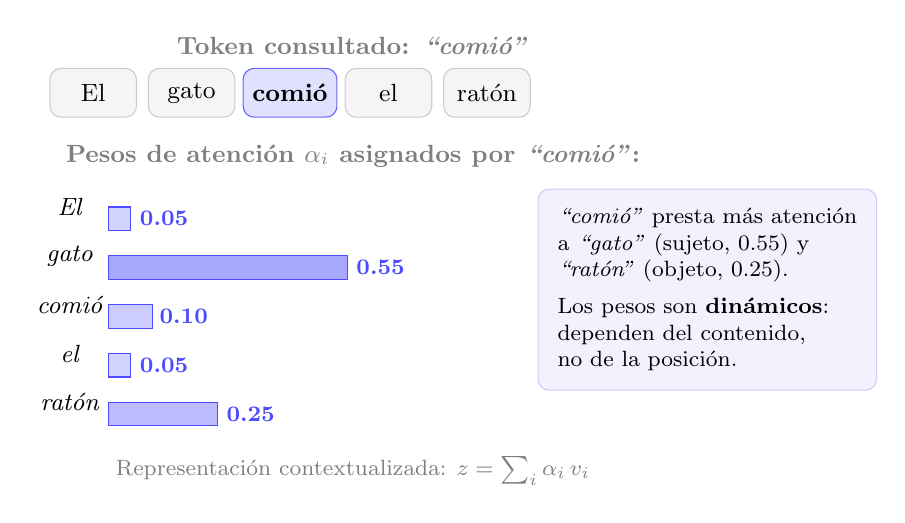
\begin{tikzpicture}[
    word/.style={draw=gray!40, rounded corners, fill=gray!8,
                 minimum width=1.1cm, minimum height=0.62cm, font=\small},
    focus/.style={draw=blue!60, rounded corners, fill=blue!12,
                  minimum width=1.1cm, minimum height=0.62cm,
                  font=\small\bfseries},
    weight/.style={font=\footnotesize\bfseries},
    bar/.style={fill=blue!50, draw=blue!70}
]

\node[font=\small\bfseries, gray] at (3.3, 5.6)
    {Token consultado: \textit{``comi\'o''}};

\node[word]  at (0*1.25, 5.0) {El};
\node[word]  at (1*1.25, 5.0) {gato};
\node[focus] at (2*1.25, 5.0) {comi\'o};
\node[word]  at (3*1.25, 5.0) {el};
\node[word]  at (4*1.25, 5.0) {rat\'on};

\node[font=\small\bfseries, gray] at (3.3, 4.2)
    {Pesos de atenci\'on $\alpha_i$ asignados por \textit{``comi\'o''}:};

\node[font=\small\itshape] at (-0.3, 3.55) {El};
\fill[bar, fill opacity=0.35] (0.2, 3.25) rectangle (0.475, 3.55);
\node[weight, blue!70] at (0.9, 3.40) {0.05};

\node[font=\small\itshape] at (-0.3, 2.93) {gato};
\fill[bar, fill opacity=0.685] (0.2, 2.63) rectangle (3.225, 2.93);
\node[weight, blue!70] at (3.65, 2.78) {0.55};

\node[font=\small\itshape] at (-0.3, 2.31) {comi\'o};
\fill[bar, fill opacity=0.40] (0.2, 2.01) rectangle (0.75, 2.31);
\node[weight, blue!70] at (1.15, 2.16) {0.10};

\node[font=\small\itshape] at (-0.3, 1.69) {el};
\fill[bar, fill opacity=0.35] (0.2, 1.39) rectangle (0.475, 1.69);
\node[weight, blue!70] at (0.9, 1.54) {0.05};

\node[font=\small\itshape] at (-0.3, 1.07) {rat\'on};
\fill[bar, fill opacity=0.525] (0.2, 0.77) rectangle (1.575, 1.07);
\node[weight, blue!70] at (2.0, 0.92) {0.25};

\node[draw=blue!20, fill=blue!5, rounded corners, font=\footnotesize,
      inner sep=7pt, align=left] at (7.8, 2.5)
    {\textit{``comi\'o''} presta m\'as atenci\'on\\
     a \textit{``gato''} (sujeto, 0.55) y\\
     \textit{``rat\'on''} (objeto, 0.25).\\[4pt]
     Los pesos son \textbf{din\'amicos}:\\
     dependen del contenido,\\
     no de la posici\'on.};

\node[font=\footnotesize, gray] at (3.3, 0.2)
    {Representaci\'on contextualizada:
     $\bm{z} = \sum_i \alpha_i \, \bm{v}_i$};

\end{tikzpicture}
\caption{Intuici\'on del mecanismo de atenci\'on. Para el token
\textit{comi\'o}, la atenci\'on calcula un peso $\alpha_i$ para cada
token de la secuencia. La representaci\'on final es una suma ponderada
de los valores, donde los pesos reflejan la relevancia sem\'antica.}
\label{fig:atencion_intuicion}
\end{figure}

% ============================================================
\begin{figure}[H]
\centering
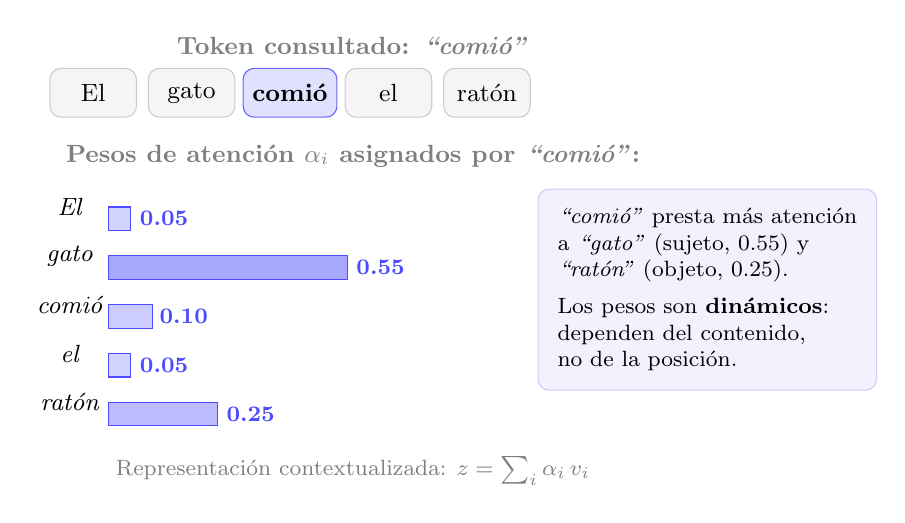
\begin{tikzpicture}[
    word/.style={draw=gray!40, rounded corners, fill=gray!8,
                 minimum width=1.1cm, minimum height=0.62cm, font=\small},
    focus/.style={draw=blue!60, rounded corners, fill=blue!12,
                  minimum width=1.1cm, minimum height=0.62cm,
                  font=\small\bfseries},
    weight/.style={font=\footnotesize\bfseries},
    bar/.style={fill=blue!50, draw=blue!70}
]

\node[font=\small\bfseries, gray] at (3.3, 5.6)
    {Token consultado: \textit{``comi\'o''}};

\node[word]  at (0*1.25, 5.0) {El};
\node[word]  at (1*1.25, 5.0) {gato};
\node[focus] at (2*1.25, 5.0) {comi\'o};
\node[word]  at (3*1.25, 5.0) {el};
\node[word]  at (4*1.25, 5.0) {rat\'on};

\node[font=\small\bfseries, gray] at (3.3, 4.2)
    {Pesos de atenci\'on $\alpha_i$ asignados por \textit{``comi\'o''}:};

\node[font=\small\itshape] at (-0.3, 3.55) {El};
\fill[bar, fill opacity=0.35] (0.2, 3.25) rectangle (0.475, 3.55);
\node[weight, blue!70] at (0.9, 3.40) {0.05};

\node[font=\small\itshape] at (-0.3, 2.93) {gato};
\fill[bar, fill opacity=0.685] (0.2, 2.63) rectangle (3.225, 2.93);
\node[weight, blue!70] at (3.65, 2.78) {0.55};

\node[font=\small\itshape] at (-0.3, 2.31) {comi\'o};
\fill[bar, fill opacity=0.40] (0.2, 2.01) rectangle (0.75, 2.31);
\node[weight, blue!70] at (1.15, 2.16) {0.10};

\node[font=\small\itshape] at (-0.3, 1.69) {el};
\fill[bar, fill opacity=0.35] (0.2, 1.39) rectangle (0.475, 1.69);
\node[weight, blue!70] at (0.9, 1.54) {0.05};

\node[font=\small\itshape] at (-0.3, 1.07) {rat\'on};
\fill[bar, fill opacity=0.525] (0.2, 0.77) rectangle (1.575, 1.07);
\node[weight, blue!70] at (2.0, 0.92) {0.25};

\node[draw=blue!20, fill=blue!5, rounded corners, font=\footnotesize,
      inner sep=7pt, align=left] at (7.8, 2.5)
    {\textit{``comi\'o''} presta m\'as atenci\'on\\
     a \textit{``gato''} (sujeto, 0.55) y\\
     \textit{``rat\'on''} (objeto, 0.25).\\[4pt]
     Los pesos son \textbf{din\'amicos}:\\
     dependen del contenido,\\
     no de la posici\'on.};

\node[font=\footnotesize, gray] at (3.3, 0.2)
    {Representaci\'on contextualizada:
     $\bm{z} = \sum_i \alpha_i \, \bm{v}_i$};

\end{tikzpicture}
\caption{Intuici\'on del mecanismo de atenci\'on. Para el token
\textit{comi\'o}, la atenci\'on calcula un peso $\alpha_i$ para cada
token de la secuencia. La representaci\'on final es una suma ponderada
de los valores, donde los pesos reflejan la relevancia sem\'antica.}
\label{fig:atencion_intuicion}
\end{figure}

% ============================================================
\begin{figure}[H]
\centering
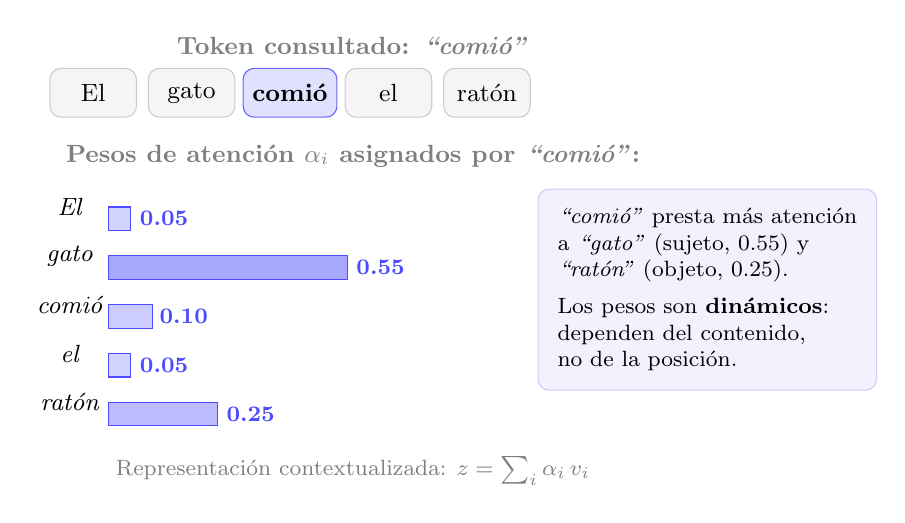
\begin{tikzpicture}[
    word/.style={draw=gray!40, rounded corners, fill=gray!8,
                 minimum width=1.1cm, minimum height=0.62cm, font=\small},
    focus/.style={draw=blue!60, rounded corners, fill=blue!12,
                  minimum width=1.1cm, minimum height=0.62cm,
                  font=\small\bfseries},
    weight/.style={font=\footnotesize\bfseries},
    bar/.style={fill=blue!50, draw=blue!70}
]

\node[font=\small\bfseries, gray] at (3.3, 5.6)
    {Token consultado: \textit{``comi\'o''}};

\node[word]  at (0*1.25, 5.0) {El};
\node[word]  at (1*1.25, 5.0) {gato};
\node[focus] at (2*1.25, 5.0) {comi\'o};
\node[word]  at (3*1.25, 5.0) {el};
\node[word]  at (4*1.25, 5.0) {rat\'on};

\node[font=\small\bfseries, gray] at (3.3, 4.2)
    {Pesos de atenci\'on $\alpha_i$ asignados por \textit{``comi\'o''}:};

\node[font=\small\itshape] at (-0.3, 3.55) {El};
\fill[bar, fill opacity=0.35] (0.2, 3.25) rectangle (0.475, 3.55);
\node[weight, blue!70] at (0.9, 3.40) {0.05};

\node[font=\small\itshape] at (-0.3, 2.93) {gato};
\fill[bar, fill opacity=0.685] (0.2, 2.63) rectangle (3.225, 2.93);
\node[weight, blue!70] at (3.65, 2.78) {0.55};

\node[font=\small\itshape] at (-0.3, 2.31) {comi\'o};
\fill[bar, fill opacity=0.40] (0.2, 2.01) rectangle (0.75, 2.31);
\node[weight, blue!70] at (1.15, 2.16) {0.10};

\node[font=\small\itshape] at (-0.3, 1.69) {el};
\fill[bar, fill opacity=0.35] (0.2, 1.39) rectangle (0.475, 1.69);
\node[weight, blue!70] at (0.9, 1.54) {0.05};

\node[font=\small\itshape] at (-0.3, 1.07) {rat\'on};
\fill[bar, fill opacity=0.525] (0.2, 0.77) rectangle (1.575, 1.07);
\node[weight, blue!70] at (2.0, 0.92) {0.25};

\node[draw=blue!20, fill=blue!5, rounded corners, font=\footnotesize,
      inner sep=7pt, align=left] at (7.8, 2.5)
    {\textit{``comi\'o''} presta m\'as atenci\'on\\
     a \textit{``gato''} (sujeto, 0.55) y\\
     \textit{``rat\'on''} (objeto, 0.25).\\[4pt]
     Los pesos son \textbf{din\'amicos}:\\
     dependen del contenido,\\
     no de la posici\'on.};

\node[font=\footnotesize, gray] at (3.3, 0.2)
    {Representaci\'on contextualizada:
     $\bm{z} = \sum_i \alpha_i \, \bm{v}_i$};

\end{tikzpicture}
\caption{Intuici\'on del mecanismo de atenci\'on. Para el token
\textit{comi\'o}, la atenci\'on calcula un peso $\alpha_i$ para cada
token de la secuencia. La representaci\'on final es una suma ponderada
de los valores, donde los pesos reflejan la relevancia sem\'antica.}
\label{fig:atencion_intuicion}
\end{figure}

% ============================================================
\begin{figure}[H]
\centering
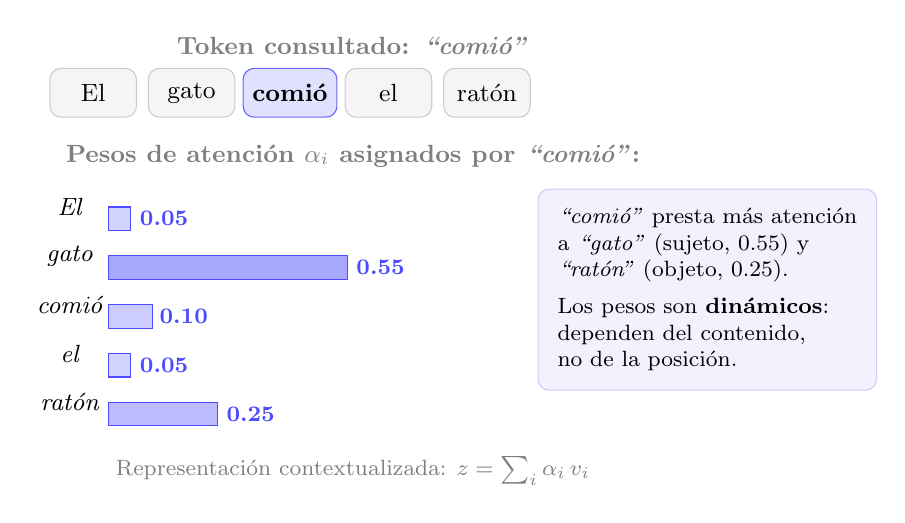
\begin{tikzpicture}[
    word/.style={draw=gray!40, rounded corners, fill=gray!8,
                 minimum width=1.1cm, minimum height=0.62cm, font=\small},
    focus/.style={draw=blue!60, rounded corners, fill=blue!12,
                  minimum width=1.1cm, minimum height=0.62cm,
                  font=\small\bfseries},
    weight/.style={font=\footnotesize\bfseries},
    bar/.style={fill=blue!50, draw=blue!70}
]

\node[font=\small\bfseries, gray] at (3.3, 5.6)
    {Token consultado: \textit{``comi\'o''}};

\node[word]  at (0*1.25, 5.0) {El};
\node[word]  at (1*1.25, 5.0) {gato};
\node[focus] at (2*1.25, 5.0) {comi\'o};
\node[word]  at (3*1.25, 5.0) {el};
\node[word]  at (4*1.25, 5.0) {rat\'on};

\node[font=\small\bfseries, gray] at (3.3, 4.2)
    {Pesos de atenci\'on $\alpha_i$ asignados por \textit{``comi\'o''}:};

\node[font=\small\itshape] at (-0.3, 3.55) {El};
\fill[bar, fill opacity=0.35] (0.2, 3.25) rectangle (0.475, 3.55);
\node[weight, blue!70] at (0.9, 3.40) {0.05};

\node[font=\small\itshape] at (-0.3, 2.93) {gato};
\fill[bar, fill opacity=0.685] (0.2, 2.63) rectangle (3.225, 2.93);
\node[weight, blue!70] at (3.65, 2.78) {0.55};

\node[font=\small\itshape] at (-0.3, 2.31) {comi\'o};
\fill[bar, fill opacity=0.40] (0.2, 2.01) rectangle (0.75, 2.31);
\node[weight, blue!70] at (1.15, 2.16) {0.10};

\node[font=\small\itshape] at (-0.3, 1.69) {el};
\fill[bar, fill opacity=0.35] (0.2, 1.39) rectangle (0.475, 1.69);
\node[weight, blue!70] at (0.9, 1.54) {0.05};

\node[font=\small\itshape] at (-0.3, 1.07) {rat\'on};
\fill[bar, fill opacity=0.525] (0.2, 0.77) rectangle (1.575, 1.07);
\node[weight, blue!70] at (2.0, 0.92) {0.25};

\node[draw=blue!20, fill=blue!5, rounded corners, font=\footnotesize,
      inner sep=7pt, align=left] at (7.8, 2.5)
    {\textit{``comi\'o''} presta m\'as atenci\'on\\
     a \textit{``gato''} (sujeto, 0.55) y\\
     \textit{``rat\'on''} (objeto, 0.25).\\[4pt]
     Los pesos son \textbf{din\'amicos}:\\
     dependen del contenido,\\
     no de la posici\'on.};

\node[font=\footnotesize, gray] at (3.3, 0.2)
    {Representaci\'on contextualizada:
     $\bm{z} = \sum_i \alpha_i \, \bm{v}_i$};

\end{tikzpicture}
\caption{Intuici\'on del mecanismo de atenci\'on. Para el token
\textit{comi\'o}, la atenci\'on calcula un peso $\alpha_i$ para cada
token de la secuencia. La representaci\'on final es una suma ponderada
de los valores, donde los pesos reflejan la relevancia sem\'antica.}
\label{fig:atencion_intuicion}
\end{figure}
